\documentclass[11pt]{scrartcl}
\usepackage[noasy]{alan}
\usepackage{booktabs}
\usepackage{graphicx}
\graphicspath{{./}{writeup/}}  % figures/ lives in docs/writeup/
\usepackage{tikz}

\setkomafont{caption}{\small}
\setlist{itemsep=2pt}
\setlength{\emergencystretch}{3em}

\newcommand{\ket}[1]{\lvert #1\rangle}
\newcommand{\bra}[1]{\langle #1\rvert}
\newcommand{\D}[2]{D^{#1}_{#2}}
\newcommand{\CZ}{\ensuremath{\mathrm{CZ}}}
\newcommand{\file}[1]{\texttt{\small #1}}

\title{Preparing Dicke States on Willow}
\subtitle{The mathematical choices behind our solution}
\author{Team Popeyes}
\date{DuQuantum $\times$ Google Quantum AI Challenge, Standard and Bonus Tracks $\cdot$ October 25, 2026}

\begin{document}
\maketitle

\begin{abstract}
  Our function \file{create\_dicke\_state} returns an exact circuit of \CZ{} and \texttt{PhasedXZ}
  gates on calibrated qubits of Google's Willow chip. The submission is \file{submission.ipynb}, the
  challenge notebook with \file{main.py} embedded verbatim. This note states the mathematical fact
  behind each design choice, with a short justification for each. \Cref{sec:bonus} covers the
  bonus track.

  We assume linear algebra (vectors, $2\times2$ matrices), first-year probability (expected value,
  variance, the normal distribution) and one-variable calculus. Every quantum notion is defined
  where it first appears. A gentler four-idea overview is in \file{docs/writeup/main.pdf}.

  Every number here is \emph{simulated} with calibrated gate errors, energy decay
  ($T_1=68\,\mu$s~\cite{willow}), dephasing ($T_\varphi=100\,\mu$s, assumed) and asymmetric readout
  errors. Nothing here has run on hardware. File paths refer to the repository.
\end{abstract}

%% ---------------------------------------------------------------------------
\section{Background and notation}

\subsection{Qubits and the Dicke state}

A \vocab{qubit} is a unit vector $a\ket0+b\ket1$ in $\CC^2$, where $\ket0$ and $\ket1$ are the two
standard basis vectors. Measuring it gives $0$ with probability $\abs a^2$ and $1$ with probability
$\abs b^2$. A state of $N$ qubits is a unit vector with one \vocab{amplitude} $\psi_b$ for each of
the $2^N$ bit strings $b$:
\[
  \ket\psi=\sum_{b\in\{0,1\}^N}\psi_b\ket b,\qquad \sum_b\abs{\psi_b}^2=1 .
\]
Measuring all qubits gives the string $b$ with probability $\abs{\psi_b}^2$. We write $\abs b$ for
the \vocab{weight} of $b$, the number of ones in it. Every state in this note has real amplitudes.

\begin{definition}[Dicke state]
  The \vocab{Dicke state} $\ket{\D Nn}$ is the equal superposition of all $N$-bit strings of weight
  $n$:
  \[
    \ket{\D Nn}=\frac{1}{\sqrt K}\sum_{\abs b=n}\ket b,\qquad K=\binom Nn .
  \]
  The case $n=1$ is the \vocab{W state} $\ket{W_N}$. We also write $k=\min(n,N-n)$.
\end{definition}

\begin{example}[$\D42$]
  $\ket{\D42}=\tfrac{1}{\sqrt6}\bigl(\ket{0011}+\ket{0101}+\ket{0110}+\ket{1001}+\ket{1010}+\ket{1100}\bigr)$,
  with $K=\binom42=6$. Measuring gives each of the six strings with probability $1/6$.
\end{example}

The circuit must produce this vector \emph{exactly}, signs included, when there is no noise.
A measurement only reveals the probabilities $\abs{\psi_b}^2$, not the signs. That is why the
judges also measure in a second basis (\Cref{sec:xterm}).

\subsection{Gates}

A \vocab{gate} is a unitary matrix applied to one or two qubits. The ones we need are
\begin{gather*}
  X=\begin{pmatrix}0&1\\1&0\end{pmatrix},\qquad
  Y=\begin{pmatrix}0&-i\\i&0\end{pmatrix},\qquad
  Z=\begin{pmatrix}1&0\\0&-1\end{pmatrix},\\
  R_y(\theta)=e^{-i\theta Y/2}=\begin{pmatrix}\cos\frac\theta2&-\sin\frac\theta2\\[2pt]\sin\frac\theta2&\cos\frac\theta2\end{pmatrix},\qquad
  \CZ=\operatorname{diag}(1,1,1,-1).
\end{gather*}
These are the \vocab{Pauli matrices} $X,Y,Z$ and the rotation generated by $Y$. $X$ flips a bit, $Z$ flips the sign of $\ket1$, and $R_y(\theta)$ rotates the real plane spanned by
$\ket0,\ket1$ by the angle $\theta/2$. The \vocab{controlled-Z} gate \CZ{} acts on two qubits and
flips the sign of $\ket{11}$ only.

The rules allow any single-qubit gate (Cirq's \texttt{PhasedXZ} gate covers every $2\times2$
unitary), but the only two-qubit gate is \CZ{}, and only between qubits that are physically
connected on the chip. A \CZ{} fails roughly ten times as often as a single-qubit gate, so a
circuit's main cost is its \vocab{CZ count}. The second cost is its \vocab{depth}, the number of
time steps (\vocab{moments}), because waiting qubits decay as well.

\subsection{The noise we simulate}

Our simulator (\file{experiments/}) uses four kinds of error:
\begin{itemize}
  \item \textbf{Gate errors.} After a gate with calibrated error rate $e$, with probability $e$ a
        random Pauli error ($X$, $Y$ or $Z$ on the qubits involved) hits the state. This model is
        called \vocab{depolarizing noise}.
  \item \textbf{Energy decay.} An idle qubit in $\ket1$ relaxes to $\ket0$ at rate $1/T_1$.
  \item \textbf{Dephasing.} An idle qubit in a superposition picks up a random sign between $\ket0$
        and $\ket1$ at rate $1/T_\varphi$.
  \item \textbf{Readout errors.} Each qubit reads 1 as 0 with probability $e^{1\to0}_q$ and 0 as
        1 with probability $e^{0\to1}_q$. The first rate is typically about twice the second.
\end{itemize}

%% ---------------------------------------------------------------------------
\section{The judges' score}

Each test case $(N,n)$ is judged from $10^4$ shots in the $Z$ basis (measure every qubit
directly) and $10^4$ in the $X$ basis (explained below). The score of the case is
\[
  S=\frac{1}{z+x},
\]
and the total is the sum of $S$ over all test cases. The pairs $(N,n)$ are not disclosed.

\subsection{The \texorpdfstring{$Z$}{Z} term: is every valid string equally likely?}

Throw away the $Z$-basis shots whose weight is not $n$. Let $f$ be the fraction that remain, let
$F=10^4f$ be their number, and let $c_b$ count the shots that gave string $b$. If the state were
perfect, each of the $K$ valid strings would be expected $F/K$ times. The judges compare the
counts with this even split using Pearson's \vocab{chi-squared statistic}:
\[
  \chi^2=\sum_{\abs b=n}\frac{(c_b-F/K)^2}{F/K},\qquad z=\frac{\chi^2}{Kf}.
\]
So $z$ is small when the counts look evenly split and when few shots were thrown away.

\subsection{The \texorpdfstring{$X$}{X} term: are the signs right?}\label{sec:xterm}

Measuring in the \vocab{$X$ basis} means applying a Hadamard gate to every qubit before reading it
out. A bit $b_i$ read this way is the outcome of the observable $X_i$, whose value is $(-1)^{b_i}$.
For a set $A$ of qubits, the product $X_A=\prod_{i\in A}X_i$ has value $(-1)^{\abs{b\cap A}}$, where
$\abs{b\cap A}$ counts the ones of $b$ inside $A$. Averaging over shots estimates the
\vocab{correlator} $\langle X_A\rangle=\bra\psi X_A\ket\psi$.

Let $\bar C_j$ be the average of $\langle X_A\rangle$ over all $\binom Nj$ subsets $A$ of size $j$,
and $C^\star_j$ its ideal value. Then
\[
  x=\sum_{j=1}^{M}\eps_j^2,\qquad
  \eps_j=\begin{cases}(\bar C_j-C^\star_j)/C^\star_j,&C^\star_j\ne0,\\ \bar C_j,&C^\star_j=0.\end{cases}
\]
$M$ is undisclosed. We report $M=N$, the strictest choice.

\begin{proposition}[Ideal correlators]
  For $\ket{\D Nn}$, $C^\star_j=\binom{j}{j/2}\binom{N-j}{n-j/2}\Big/\binom Nn$ when $j$ is even, and
  $C^\star_j=0$ when $j$ is odd.
\end{proposition}
\begin{proof}
  $X_A$ flips the bits in $A$, so $X_A\ket s=\ket{s\oplus A}$. Then
  \[
    \bra{\D Nn}X_A\ket{\D Nn}=\frac1K\sum_{\abs s=n}\,\sum_{\abs t=n}\langle t\vert s\oplus A\rangle,
  \]
  and the inner sum is 1 exactly when $s\oplus A$ again has weight $n$. If $s$ has $i$ ones inside
  $A$, flipping $A$ changes the weight by $j-2i$, so the weight is kept exactly when $i=j/2$. That is
  impossible for odd $j$. For even $j$, the number of such $s$ is $\binom{j}{j/2}$ (choose which
  half of $A$ is ones) times $\binom{N-j}{n-j/2}$ (place the other ones outside $A$).
\end{proof}

\begin{example}
  For $\ket{\D42}$: $C^\star_2=\binom21\binom21/6=2/3$ and $C^\star_4=\binom42/6=1$. The second
  value says that flipping all four bits maps $\ket{\D42}$ to itself, which is the complement
  symmetry of \Cref{sec:reductions}.
\end{example}

\subsection{Fast scoring}

Evaluating $x$ directly means averaging over all $\binom Nj$ subsets for every shot. A counting
argument removes that cost.

\begin{claim*}
  For one $X$-basis shot $b$ of weight $w$, the average of $(-1)^{\abs{b\cap A}}$ over all $j$-subsets
  $A$ is $\mathcal K_j(w)/\binom Nj$, where
  $\mathcal K_j(w)=\sum_i(-1)^i\binom wi\binom{N-w}{j-i}$ is a \vocab{Krawtchouk polynomial}.
\end{claim*}
\begin{proof}
  A subset $A$ with $i$ of its $j$ elements among the $w$ ones of $b$ contributes $(-1)^i$. There
  are $\binom wi\binom{N-w}{j-i}$ such subsets.
\end{proof}

So $x$ depends only on the histogram of shot weights, not on the strings themselves. That is
what makes 20{,}000 simulated judged runs per case cheap (\file{experiments/scoring.py}).

%% ---------------------------------------------------------------------------
\section{The score is heavy-tailed: small \texorpdfstring{$K$}{K} and uniformity come first}\label{sec:score}

The score is the \emph{reciprocal} of a random quantity. If $z$ is usually about 1 but
occasionally lands very close to 0, then $S$ is usually about 1 but occasionally enormous. Those
rare large values dominate the average. This section makes that precise.

\subsection{The chi-squared distribution}

\begin{definition}
  If $G_1,\dots,G_\nu$ are independent standard normal variables, the distribution of
  $G_1^2+\dots+G_\nu^2$ is the \vocab{chi-squared distribution with $\nu$ degrees of freedom},
  $\chi^2_\nu$. Its density on $t>0$ is
  \[
    p_\nu(t)=\frac{t^{\nu/2-1}e^{-t/2}}{2^{\nu/2}\,\Gamma(\nu/2)},
  \]
  where $\Gamma$ is the gamma function, $\Gamma(s)=\int_0^\infty t^{s-1}e^{-t}\,dt$, which satisfies
  $\Gamma(s+1)=s\,\Gamma(s)$.
\end{definition}

\begin{fact}
  For a perfect state and many shots, Pearson's statistic $\chi^2$ follows $\chi^2_{K-1}$.
\end{fact}

Each term $(c_b-F/K)/\sqrt{F/K}$ is approximately normal, by the central limit theorem. The $K$
counts must add up to $F$, which removes one independent direction, so $K-1$ degrees of freedom
remain.

\begin{lemma}\label{lem:inv}
  $\EE[1/\chi^2_\nu]=1/(\nu-2)$ for $\nu>2$, and $\EE[1/\chi^2_\nu]=\infty$ for $\nu\le2$.
\end{lemma}
\begin{proof}
  Near $t=0$ the integrand $p_\nu(t)/t$ behaves like $t^{\nu/2-2}$, which is integrable exactly when
  $\nu/2-2>-1$, that is, $\nu>2$. In that case, the integral $\int_0^\infty t^{\nu/2-2}e^{-t/2}\,dt$
  is the same as in the normalization of $p_{\nu-2}$, so
  \[
    \EE[1/\chi^2_\nu]=\frac{2^{(\nu-2)/2}\,\Gamma(\nu/2-1)}{2^{\nu/2}\,\Gamma(\nu/2)}
    =\frac{1}{2\,(\nu/2-1)}=\frac{1}{\nu-2}.\qedhere
  \]
\end{proof}

\subsection{Expected score of a perfect state}

With $f$ and $x$ held fixed, $S=1/\bigl(\chi^2/(Kf)+x\bigr)=Kf/(\chi^2+a)$ with $a=Kfx$. So
\[
  \EE[S]=Kf\,\EE\!\left[\frac{1}{\chi^2_{K-1}+a}\right]\approx
  \begin{cases}
    \dfrac{Kf}{K-3}, & K>3,\\[8pt]
    \tfrac32 f\,e^{a/2}E_1(a/2)\;\approx\;\tfrac32 f\bigl(\ln\tfrac2a-\gamma\bigr), & K=3,\\[6pt]
    2f\sqrt{\pi/(2a)}\;\operatorname{erfcx}\!\sqrt{a/2}\;\approx\;\sqrt{\pi f/x}, & K=2.
  \end{cases}
\]
Here $E_1(u)=\int_u^\infty e^{-t}/t\,dt$ is the \vocab{exponential integral}, $\gamma\approx0.577$
is Euler's constant, and $\operatorname{erfcx}(u)=e^{u^2}\operatorname{erfc}(u)$ is the scaled
complementary error function. Both of the last two are close to their small-$a$ forms because $a$
is tiny.
\begin{itemize}
  \item \textbf{$K>3$.} This follows from \Cref{lem:inv} with $\nu=K-1>2$, ignoring the small $a$.
        The mean is finite even at $x=0$.
  \item \textbf{$K=3$.} Here $p_2(t)=\tfrac12e^{-t/2}$, and substituting $u=(t+a)/2$ gives
        $\int_0^\infty\frac{e^{-t/2}}{2(t+a)}\,dt=\tfrac12e^{a/2}E_1(a/2)$ exactly. For small $u$,
        $E_1(u)\approx-\ln u-\gamma$.
  \item \textbf{$K=2$.} Here $p_1(t)=e^{-t/2}/\sqrt{2\pi t}$. Substituting $t=u^2$ turns the integral
        into the standard form $\int_0^\infty e^{-u^2/2}/(u^2+a)\,du$, which gives the erfcx expression
        exactly. Since $\operatorname{erfcx}(0)=1$, the score grows like $x^{-1/2}$ as $x\to0$.
\end{itemize}
For $K\le3$, \Cref{lem:inv} says the mean would be infinite at $x=0$. Only the $X$ term keeps it
finite.

\begin{center}\small
\begin{tabular}{lcccccc}
  \toprule
  $K$ & 2 & 3 & 4 & 6 & 10 & 20\\
  \midrule
  $\EE[S]$, perfect state, $f=0.9$, $x=10^{-3}$ & 51.4 & 8.15 & 3.34 & 1.79 & 1.28 & 1.06\\
  \bottomrule
\end{tabular}\\[2pt]
At $K=2$: $x=10^{-4}$ gives 166 and $x=10^{-2}$ gives 15.2 (\file{scoring.expected\_score}).
\end{center}

A single $K=2$ case, such as $W_2$, is worth about fifty large cases.

\subsection{Imbalance removes the tail}

Suppose valid string $b$ appears with probability $(1+\delta_b)/K$ inside the subspace instead
of $1/K$. Then each term of $\chi^2$ is a squared normal with a nonzero mean. Such a sum follows
the \vocab{noncentral chi-squared distribution}, whose \vocab{noncentrality} $\lambda$ is the sum
of the squared means:
\[
  \lambda=\sum_b\frac{\bigl(F(1+\delta_b)/K-F/K\bigr)^2}{F/K}=F\,\overline{\delta^2}=10^4 f\,\overline{\delta^2},
\]
where $\overline{\delta^2}$ is the average of $\delta_b^2$ over the $K$ strings. The mean becomes
$\EE[\chi^2]=K-1+\lambda$, so $z$ grows by about $10^4\,\overline{\delta^2}/K$. More importantly,
$\chi^2$ can no longer land near 0, so the lucky draws disappear.

\begin{example}
  A 1\% rms imbalance ($\delta_{\mathrm{rms}}=0.01$, so $\lambda\approx0.9$) lowers $\EE[S]$ at $K=2$
  from 51.4 to 33.3, and a 3\% imbalance ($\lambda\approx8$) lowers it to 1.3. At $K=4$ the same
  steps give 3.34, 2.53 and 0.53.
\end{example}

\begin{figure}[h]
  \centering
  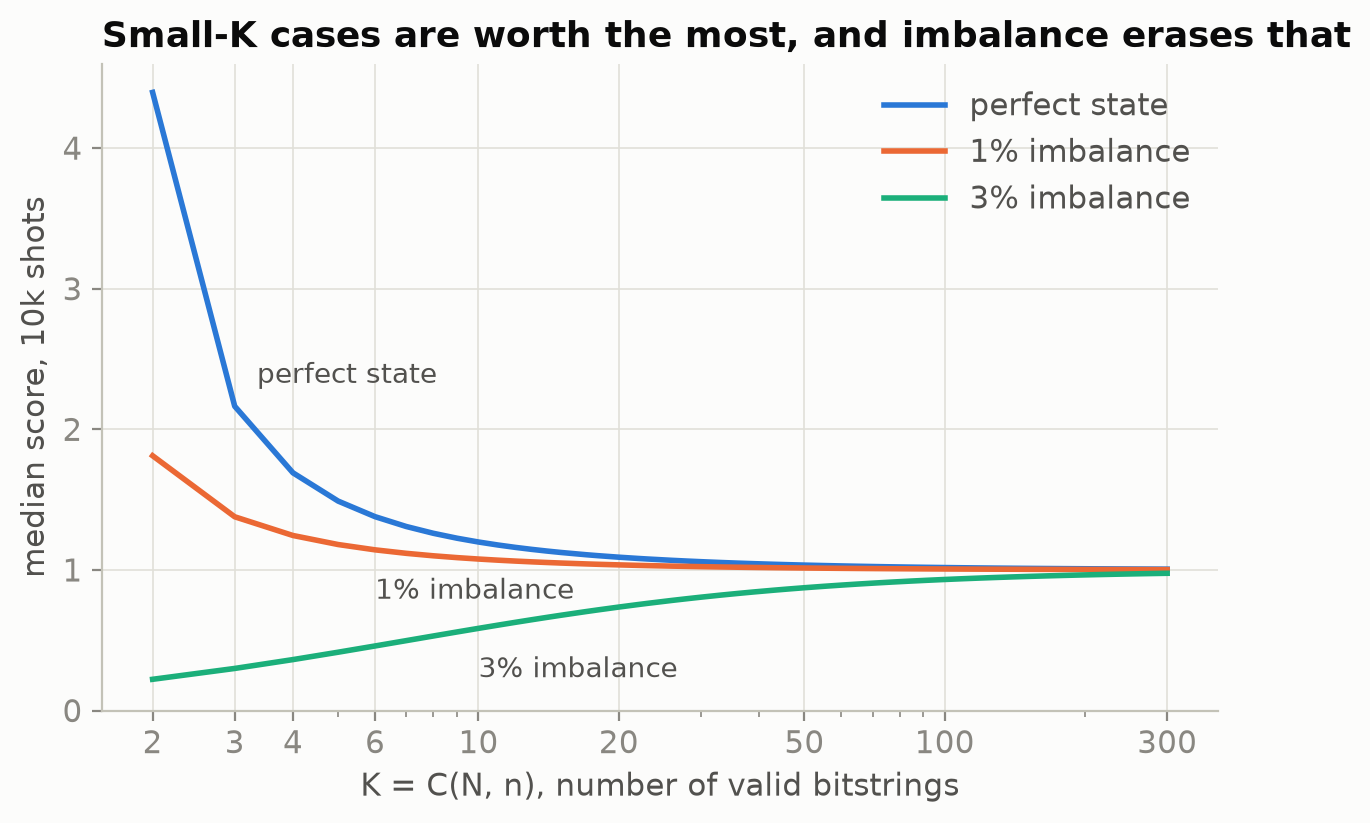
\includegraphics[width=0.48\linewidth]{figures/score_tail.png}\hfill
  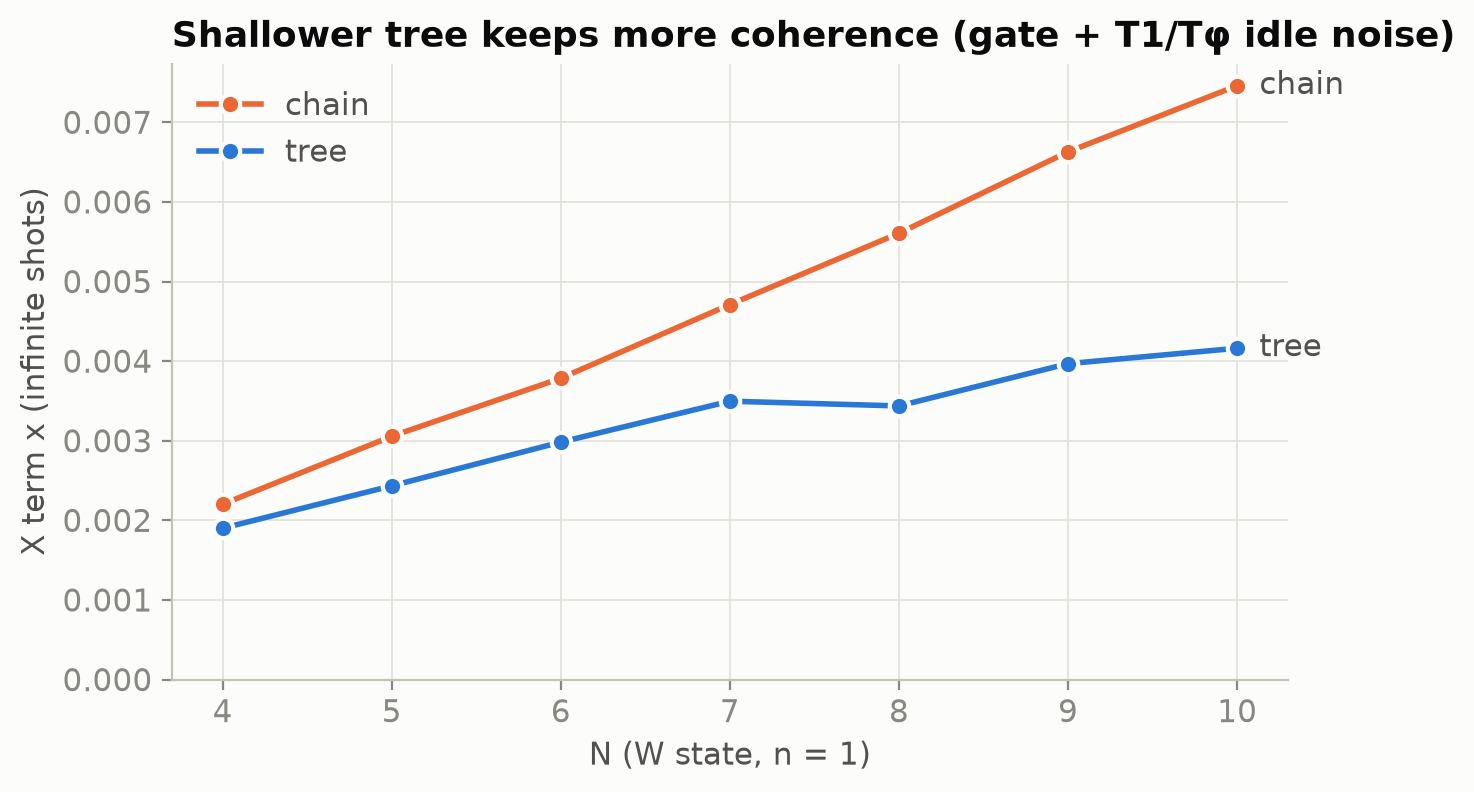
\includegraphics[width=0.48\linewidth]{figures/tree_vs_chain.png}
  \caption{Left: median single-draw score versus $K$ for a perfect state and for 1\% and 3\% rms
    imbalance. Right: $X$ term of $W_N$ under gate and idle noise, tree versus chain
    (\file{w\_tree.csv}, \Cref{sec:w}).}
\end{figure}

\begin{remark}[Consequences]
  What this means for the design:
  \begin{itemize}
    \item The judges sum single draws, so our objective is $\sum\EE[S]$. We compute it by
          integrating $1/(z+x)$ against the noncentral $\chi^2$ density numerically, with $x$
          held at its mean. Averaging resampled runs does not work at $K\le3$, where a few lucky
          draws dominate the average.
    \item Priority order: a valid circuit on every case, since any valid circuit scores above 0;
          then uniformity ($\delta_{\mathrm{rms}}\lesssim1\%$) and a low $x$ floor at small $K$; then the
          fraction $f$ of valid shots, which costs only $1/f$; then coherence at large $N$.
    \item We may not pre-compensate known biases by tilting the amplitudes, because the noiseless
          state must be exact. Uniformity can only come from the construction and from the choice
          of qubits.
  \end{itemize}
\end{remark}

\subsection{The organizers' revised preliminary ranking}

On October 25 the organizers changed the preliminary leaderboard. It now averages $1/S$ over
trials and reports $1/\overline{1/S}=1/\EE[z+x]$, because the plain mean diverges as the noise
vanishes (\Cref{lem:inv}). With $\EE[\chi^2]=K-1+\lambda$,
\[
  \frac{1}{\EE[z+x]}=\frac{1}{\dfrac{K-1+\lambda}{Kf}+x}\approx\frac{1}{\dfrac1f+\dfrac{\lambda}{Kf}+x}
  \qquad(K\gg1).
\]
This removes the heavy tail. The organizers tested $\D{10}3$, $\D{10}5$ and $\D{15}4$, with
$K=120$, 252 and 1365. For those the score is set by the total error budget through $f$ and by
coherence through $x$; imbalance enters only as $\lambda/K$. On that ranking our first submission
led on $\D{10}3$ and trailed the teammates' preliminary combined submission on $\D{10}5$ and
$\D{15}4$. The error budgets traced the gap to dense single-qubit pulses (\Cref{sec:compile}). The
notebook still describes final judging as one draw per case on hardware, so $\sum\EE[S]$ stays our
objective and we report $1/\EE[z+x]$ next to it.

%% ---------------------------------------------------------------------------
\section{Two free reductions}\label{sec:reductions}

\textbf{Complement.} $X^{\otimes N}\ket{\D Nn}=\ket{\D N{N-n}}$, because flipping every bit maps
weight-$n$ strings one-to-one onto weight-$(N-n)$ strings. So we only build $n=k\le N/2$, and the
final layer of $X$ gates merges into the last single-qubit gates at no cost.

\textbf{Permutation symmetry.} Swapping two qubits maps $\ket{\D Nn}$ to itself, and the returned
qubits are a set, not an ordered list. So any placement of a construction's shape on the chip is a
valid answer, and qubit order never has to be restored after routing.

%% ---------------------------------------------------------------------------
\section{W states (\texorpdfstring{$k=1$}{k=1}): a broadcast tree with \texorpdfstring{$2N-3$}{2N-3} CZ}\label{sec:w}

A W state has a single excitation (one ``1'') shared evenly among $N$ qubits. Think of it as
probability 1 that must be split into $N$ equal shares of $1/N$.

\subsection{Construction}

\begin{algorithm*}
  Choose a spanning tree of the chosen qubits with root $r$, and let $s(v)$ be the number of qubits
  in the subtree under $v$ (including $v$). Start with $r$ in $\ket1$ and the rest in $\ket0$. In
  each round, every qubit $v$ that currently holds probability $m_v/N$ hands one child $c$ the
  fraction $p=s(c)/m_v$ of it, using the two-qubit \vocab{transfer}
  \[
    \ket1_v\ket0_c\mapsto\sqrt{1-p}\,\ket{10}+\sqrt p\,\ket{01},\qquad \ket{00}\mapsto\ket{00}.
  \]
\end{algorithm*}

Afterwards $c$ holds $s(c)/N$, exactly what its subtree needs, and $v$ keeps $(m_v-s(c))/N$. By
induction every qubit ends with exactly $1/N$. Every branch of the superposition carries one
excitation, and all amplitudes stay real and positive, so the output is exactly $\ket{W_N}$.

\begin{example}[$W_4$ in two rounds]
  Take the four-qubit tree below, rooted at $r$.
  \begin{center}
  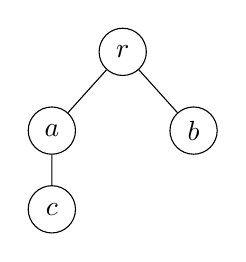
\begin{tikzpicture}[every node/.style={circle,draw,minimum size=6mm,inner sep=0pt},
      level distance=10mm, sibling distance=18mm]
    \node {$r$} child {node {$a$} child {node {$c$}}} child {node {$b$}};
  \end{tikzpicture}
  \end{center}
  Round 1: $r$ holds everything and gives $a$ the fraction $p=s(a)/4=1/2$.
  Round 2, both at once: $r$ gives $b$ half of its share, and $a$ gives $c$ half of its share.
  Every qubit now holds $1/4$. A line $r-a-c-b$ would need three rounds.
\end{example}

\subsection{Cost}

The very first transfer acts on a known product input $\ket1_v\ket0_c$. An $R_y$ rotation on $c$
gives $\ket1(\sqrt{1-p}\ket0+\sqrt p\ket1)$, and a CNOT from $c$ to $v$ (one \CZ{} between
Hadamards) turns it into $\sqrt{1-p}\ket{10}+\sqrt p\ket{01}$. That costs 1 \CZ.

Every later transfer must act correctly on both $\ket{00}$ and $\ket{10}$, because $v$ holds the
excitation only in some branches. A gate that rotates within the span of $\ket{01},\ket{10}$ and
leaves $\ket{00},\ket{11}$ alone is called a \vocab{Givens rotation}. It costs 2 \CZ{}, and one is
not enough:

\begin{claim}
  No circuit with a single \CZ{} performs the transfer with $0<p<1$.
\end{claim}
\begin{proof}
  First, a \CZ{} applied to a product state $(\alpha\ket0+\beta\ket1)\ket\phi$ gives
  $\alpha\ket0\ket\phi+\beta\ket1Z\ket\phi$. That is again a product state exactly when
  $\alpha\beta=0$ or $Z\ket\phi\propto\ket\phi$. In words: exactly when one of the two inputs is
  $\ket0$ or $\ket1$ up to a phase.

  A one-\CZ{} circuit has the form $(A_1\otimes B_1)\,\CZ\,(A_0\otimes B_0)$, and the outer
  single-qubit gates $A_1\otimes B_1$ cannot create or remove entanglement. The transfer must keep
  $\ket{00}$ a product state but entangle $\ket{10}$. Before the \CZ{}, these inputs have become
  $A_0\ket0\otimes B_0\ket0$ and $A_0\ket1\otimes B_0\ket0$. If $B_0\ket0$ is a basis state, both
  stay products. Otherwise $A_0\ket0$ must be a basis state, which forces the orthogonal vector
  $A_0\ket1$ to be one too, and again both stay products. Either way $\ket{10}$ is not entangled, a
  contradiction. (Bryan's argument, \file{docs/bryan\_constructions.md}.)
\end{proof}

The total is $1+2(N-2)=2N-3$ \CZ. An exhaustive search shows this is optimal for $W_3$ (3 \CZ) and
$W_4$ (5 \CZ).

\subsection{Why a tree}

A chain (line) has the same \CZ{} count but $N-1$ sequential transfers. The tree runs the transfers
of a round in parallel, so the number of rounds grows roughly like $\log_2 N$. $W_{10}$ takes 15
moments instead of 37, and under idle noise $x$ drops from 0.0075 to 0.0042. The circuit also
preserves the number of excitations, so every branch spends the same time in $\ket1$. Energy decay
then lowers every valid string equally and creates no imbalance.

\subsection{The smallest cases}

For $W_2$ ($K=2$) the score is set by $x$ and $\lambda$, not by \CZ{} count (\Cref{sec:score}). We
simulate every candidate qubit pair under the calibrated noise and keep the one with the highest
predicted $\EE[S]$. That gives $+9\%$ expected score and $-5\%$ median score, a deliberate trade
toward the objective.

%% ---------------------------------------------------------------------------
\section{Whole-state synthesis for \texorpdfstring{$N\le8$}{N <= 8}}\label{sec:synth}

The general construction (\Cref{sec:be}) uses gates between qubits that are not neighbours on the
chip, and fixing that adds many \CZ{}s. For small $N$ we let a computer search for an exact circuit
instead.

\subsection{The template}

The circuit alternates $L+1$ layers of $R_y$ rotations, one angle per qubit per layer, with $L$
layers of \CZ{} gates. The \CZ{}s come from a fixed shape on the chip: a path, or a $2\times m$
patch of the grid (a ladder). The edges of the shape are split into \vocab{matchings}, sets of edges
that share no qubit, so the \CZ{}s of one layer can run at the same time. This is the
\vocab{brickwork} pattern.

\textbf{Why only $R_y$.} Dicke amplitudes are real, and $R_y$ and \CZ{} are real matrices, so the
search never leaves real vectors. The restriction costs no generality. Möttönen et al.~\cite{mottonen05}
show that any real state can be prepared from $R_y$ gates and CNOTs, and their CNOTs serve only to
turn a rotation around via $XR_y(\theta)X=R_y(-\theta)$. The identity $ZR_y(\theta)Z=R_y(-\theta)$
does the same job, so each CNOT can be replaced by a \CZ{}. Given enough connectivity, $R_y$ and \CZ{}
therefore reach every real state.

\subsection{The search}

Write $\ket{\psi(\theta)}$ for the output, which depends on the list of angles $\theta$. The circuit
is exact when the \vocab{infidelity}
\[
  \mathcal L(\theta)=1-\langle \D Nn\vert\psi(\theta)\rangle^2
\]
is 0, since two unit vectors have overlap $\pm1$ only when they are equal up to sign. We minimize
$\mathcal L$ with L-BFGS, a gradient method that builds an estimate of the curvature from recent
gradients, until $\mathcal L<10^{-13}$ (exact to machine precision). The gradient is computed exactly
by backpropagation through the circuit, using
\[
  \frac{d}{d\theta}R_y(\theta)=\tfrac12R_y(\theta+\pi),
\]
which follows from $\cos(\tfrac\theta2+\tfrac\pi2)=-\sin\tfrac\theta2$ and
$\sin(\tfrac\theta2+\tfrac\pi2)=\cos\tfrac\theta2$.

We start at the smallest brickwork depth that becomes exact. Then we delete single \CZ{}s greedily,
re-solve from the previous angles, and keep a deletion only if the circuit becomes exact again
(\file{experiments/synth.py}).

\begin{center}\small
\begin{tabular}{lcccccc}
  \toprule
  case & $\D42$ & $\D52$ & $\D63$ & $\D73$ & $\D83$ & $\D84$\\
  \midrule
  CZ, synthesized & 5 & 10 & 15 & 18 & 30 & 26\\
  CZ, routed B-E baseline & 21 & 35 & 80 & 98 & 123 & 162\\
  \bottomrule
\end{tabular}
\end{center}

The $\D73$, $\D83$ and $\D84$ circuits come from our teammates' longer runs of the same template on
Bridges-2 (more seeds, and a $2\times4$ patch for $\D73$ and $\D83$). They replaced our 25, 31 and
27 \CZ{} and raise $1/\EE[z+x]$ by 0.6--3.7\% on three calibrations (\file{psc\_hw*.csv}). Their
9-\CZ{} $\D52$ and 14-\CZ{} $\D63$ were not adopted: $\D52$ gained only 0.8\% and would lose its
robust angle pick (below), and $\D63$ measured 3\% worse under idle noise.

\textbf{No approximate shortcuts.} Deleting any single \CZ{} from a deployed pattern and
refitting leaves an infidelity of $3\times10^{-3}$ or worse for $\D42$, $\D52$, $\D62$ and $\D63$
(\file{vqe\_gap.csv}). Approximate circuits are not allowed anyway, so fewer \CZ{}s can only come
from a different pattern, which takes a new random start, not a deletion. Synthesis takes minutes
to hours, so the angles are cached in \file{main.py}. Placement on the chip (8 grid symmetries
$\times$ translations) happens at build time.

\subsection{Choosing among exact angle sets}

One \CZ{} pattern usually admits many exact angle sets. They behave the same under our noise model
but differ under \vocab{coherent errors}, small systematic mistakes such as a rotation that is
always 1\% too large. Our noise model does not include these, so we analyse them separately.

\begin{claim}
  In a real circuit, a small $R_y$ over-rotation by $\eps$ moves the measured probabilities by
  $O(\eps)$, but a stray $Z$ phase or a \CZ{} phase error moves them only by $O(\eps^2)$.
\end{claim}
\begin{proof}
  Insert $e^{-i\eps G}\approx I-i\eps G$ somewhere in the circuit. The state changes from the real
  vector $\psi$ to $\psi-i\eps G\psi$ to first order.
  \begin{itemize}
    \item Over-rotation: $G\propto Y$, and $-iY$ is a real matrix. The change is real, so it adds
          directly to the real amplitudes and the probabilities $\psi_b^2$ move at first order.
    \item Phase errors: $G$ is real and diagonal, so $-i\eps G\psi$ is $i$ times a real vector. Then
          $\abs{\psi_b-i\eps(G\psi)_b}^2=\psi_b^2+\eps^2(G\psi)_b^2$, and the first-order term
          vanishes.\qedhere
  \end{itemize}
\end{proof}

On the deployed $\D42$, shrinking $\eps$ from $10^{-2}$ to $10^{-3}$ cuts the population error
$10\times$ for over-rotation and $100\times$ for stray $Z$, as the claim predicts. So the choice only
models over-rotation.

For a candidate angle set $c$, let $\lambda_c$ be the imbalance it produces under a 1\%
over-rotation. Since $\delta\propto\sigma$ at first order, the imbalance scales like $\sigma^2$, so
at over-rotation $\sigma$ the expected loss is
\[
  L(c,\sigma)=\EE[\mathrm{loss}]_c+\lambda_c\,(\sigma/1\%)^2/(Kf),
\]
by the $\lambda/(Kf)$ term of \Cref{sec:score}. We do not know $\sigma$, so we compare candidates by
their \vocab{regret}, how much worse each is than the best candidate for that $\sigma$, and deploy
the \vocab{minimax-regret} choice, whose worst-case regret over
$\sigma\in\{0,0.1,0.2,0.3,0.5,1\}\%$ is smallest:
\[
  c^\star=\arg\min_c\,\max_\sigma\Bigl[L(c,\sigma)-\min_d L(d,\sigma)\Bigr].
\]
It is chosen on calibration seed 0 and checked on seeds 1--2. Sensitivity to 1\% over-rotation drops
1.1--5.5$\times$ ($\D52$: $\lambda$ from 50 to 9). Under our standard noise model, which has no
over-rotation, the change in ceiling share (expected score as a percentage of a perfect state's) is
between $-0.9$ and $+2.6$ points.

On the hardware path these picks are deployed for $\D42$, $\D52$ and $\D63$. ($\D N2$ with $N\ge6$
goes to Bryan's circuits, \Cref{sec:bryan}.) The three adopted circuits $\D73$, $\D83$, $\D84$ run
without one: each is a single exact angle set, and we have no alternatives on their structures to
choose from.

%% ---------------------------------------------------------------------------
\section{Bärtschi--Eidenbenz with synthesized SCS blocks}\label{sec:be}

\subsection{The recursion}

Sort the strings of $\ket{\D mr}$ by their last bit. A fraction $r/m$ of them end in 1, and the rest
of such a string is a weight-$(r-1)$ string on $m-1$ bits. The others end in 0. So
\[
  \ket{\D mr}=\sqrt{r/m}\,\ket{\D{m-1}{r-1}}\ket1+\sqrt{(m-r)/m}\,\ket{\D{m-1}r}\ket0 .
\]
Bärtschi and Eidenbenz~\cite{be19} turn this identity into a circuit. Start from the sorted string
$\ket{0^{N-k}1^k}$. The block $\mathrm{SCS}_m$ (``split and cyclic shift'') decides the bit at
position $m$ with the right probability and leaves a sorted string on the first $m-1$ positions.
Applying $\mathrm{SCS}_N,\mathrm{SCS}_{N-1},\dots,\mathrm{SCS}_2$ gives $\ket{\D Nk}$. Block
$\mathrm{SCS}_m$ touches only the window of positions $m-k,\dots,m$.

\subsection{Each block only needs to be right on a few inputs}

Before step $m$, the first $m$ positions hold a sorted string, so the window ($w=k+1$ qubits) only
ever sees the inputs $\ket{0^{w-l}1^l}$ with $l=0,\dots,k$, plus $\ket{1^w}$ when the window is the
whole register. On these inputs the block must act as
\[
  \ket{0^{w-l}1^l}\mapsto\sqrt{l/m}\,\ket{0^{w-l}1^l}+\sqrt{(m-l)/m}\,\ket{0^{w-l-1}1^l0}
  \quad(1\le l\le k,\ l<m),
\]
and fix $l=0$ and $l=m$. Either the last bit stays 1 (probability $l/m$), or the block of ones
shifts left and a 0 lands at position $m$. So each block is only an \vocab{isometry}: a
length-preserving map specified on a $(k+1)$- or $(k+2)$-dimensional subspace, not a full unitary
on all $2^{k+1}$ inputs. The rest of the matrix is free, which leaves room for cheaper circuits.

\subsection{Synthesis of the blocks}

We fit each block on $k+1$ consecutive path qubits with the template and pruning of
\Cref{sec:synth}. With $B$ input--output pairs $(\mathrm{in}_b,\mathrm{out}_b)$, the loss is
\[
  1-\Bigl(\tfrac1B\textstyle\sum_b\bra{\mathrm{out}_b}U\ket{\mathrm{in}_b}\Bigr)^2 .
\]
Each overlap is at most 1 in absolute value, so the loss vanishes only when every input is mapped
correctly \emph{with a common sign}. A separate sign per input would not be good enough: a
superposition of inputs, which is what the block actually receives, would then come out with wrong
relative signs.

For $k\le4$ the \CZ{} pattern is pruned once per $k$ and the angles are refit for every $m$; at $k=5$
some $m$ got their own pattern. The whole B-E circuit is then nearest-neighbour on a path and needs
no routing. Inner blocks cost 2, 4, 12 and 17 \CZ{} for $k=1,\dots,4$ and 22--29 for $k=5$, so $\D N2$
costs about $4N$ \CZ{} (\file{experiments/scs\_synth.py}). Blocks exist for $m\le20$. On the hardware
track these circuits are only a fallback, for $9\le N\le20$ when Bryan's builder (\Cref{sec:bryan})
fails; beyond $N=20$ the last resort is the routed B-E circuit.

%% ---------------------------------------------------------------------------
\section{Placement: the cost is \texorpdfstring{$\log\EE[z]$}{log E[z]}}

Willow's qubits and couplers differ a lot in quality, and by permutation symmetry
(\Cref{sec:reductions}) a circuit can go anywhere its shape fits. So we score every placement and
keep the best one.

\subsection{The cost of a placement}

From \Cref{sec:score}, $\EE[z]\approx(K-1+\lambda)/(Kf)$, so
\[
  \log\EE[z]\approx\mathrm{const}-\log f+\log\bigl(1+\lambda/(K-1)\bigr).
\]
Approximate $f$ by the probability that no error happens anywhere, $f\approx\prod(1-e)$ over all
error locations. Since $\log(1-e)\approx-e$ for small $e$, $-\log f\approx\sum e$: the product
becomes a sum, which is easy to optimize over. A placement's cost is therefore
\[
  C=\sum_{(q,q')}u_{qq'}\,e^{\CZ}_{qq'}+\sum_q\Bigl[g_q\,e^{1q}_q+\bigl(1-\tfrac nN\bigr)e^{0\to1}_q+\tfrac nN\,e^{1\to0}_q\Bigr]
  +\tau\Bigl(\tfrac1{T_1}+\tfrac1{T_\varphi}\Bigr)+\log\Bigl(1+\frac{\lambda_{\mathrm{ro}}}{K-1}\Bigr).
\]
\begin{itemize}
  \item $u_{qq'}$ is the number of \CZ{}s on coupler $(q,q')$, and $e^{\CZ}_{qq'}$ its error rate.
  \item $g_q$ is the number of single-qubit gates on qubit $q$, and $e^{1q}_q$ their error rate.
  \item Each qubit of $\ket{\D Nn}$ reads 1 with probability $n/N$, so its readout error is weighted
        accordingly. This matters because $1\to0$ errors are about twice as frequent as $0\to1$.
  \item $\tau$ is the total idle time. Decay over time $\tau$ has probability
        $1-e^{-\tau/T}\approx\tau/T$.
  \item $\lambda_{\mathrm{ro}}$ is the imbalance caused by readout, derived next.
\end{itemize}

\subsection{Readout imbalance}

A valid string $b$ is read correctly with probability
\[
  \prod_{i\in b}(1-e^{1\to0}_i)\prod_{i\notin b}(1-e^{0\to1}_i)\approx c\,\exp\Bigl(-\sum_{i\in b}d_i\Bigr),
  \qquad d_i=e^{1\to0}_i-e^{0\to1}_i,
\]
where $c=\prod_i(1-e^{0\to1}_i)$ does not depend on $b$. Strings whose ones sit on ``leaky'' qubits
(large $d_i$) are undercounted. To first order, $\delta_b\approx-\sum_{i\in b}(d_i-\bar d)$.

For a random choice of the $n$ positions of the ones, this is a sum of $n$ values drawn without
replacement from the $N$ values $d_i-\bar d$. Its variance is $\tfrac{n(N-n)}{N-1}\mathrm{Var}(d)$,
the standard formula for sampling without replacement, so
\[
  \lambda_{\mathrm{ro}}=10^4 f\,\frac{n(N-n)}{N-1}\,\mathrm{Var}(d)
\]
(\file{main.\_readout\_lambda}). A random layout gives $\delta_{\mathrm{rms}}\approx0.6\%$. Since
amplitudes cannot be pre-compensated, qubit choice is the only remedy.

\subsection{Winner's curse}

The calibrated rates are noisy estimates. If we pick the placement with the lowest \emph{estimated}
cost among many, we tend to pick one whose errors happen to be underestimated, so the minimum is
biased low. To counter this, every calibrated rate enters as value $+1\sigma$, its estimate plus one
standard uncertainty. This changed none of 75 placements on the notebook's calibrations, where every
qubit has the same uncertainty. It matters only when uncertainties differ between qubits.

%% ---------------------------------------------------------------------------
\section{Compilation}\label{sec:compile}

Every moment of our circuits is either all-\CZ{} or all-single-qubit.

\subsection{Single-qubit merge pass}

Every circuit we return, Bryan's included (\Cref{sec:bryan}), goes through one final exact pass. On
each qubit, a run of single-qubit gates between two of its two-qubit gates is replaced by the
product of the run as one \texttt{PhasedXZ} gate, or dropped if that product is the identity up to a
phase. The merged gate sits in the moment of the run's last gate, and empty moments are then
removed.

The pass is exact because a run of gates and its matrix product are the same operation. No gate
moves earlier, so no qubit leaves $\ket0$ sooner, and the moment count can only fall.

\textbf{Why it matters.} Each gate adds its own error. Bryan's constructions place a $\pi$ pulse in
every idle single-qubit slot (a dense echo sequence known as CPMG). At $N\ge9$ these made up 60\% of
their single-qubit gates. Under depolarizing noise each pulse only adds its error rate, and on
$\D{15}4$ the single-qubit error budget was as large as the \CZ{} budget ($\sum e=0.33$ against
$0.27$). The pass cuts $\D{15}4$ from 777 single-qubit gates to 276, $\D{10}5$ from 371 to 230 and
$\D94$ from 286 to 170. Measured by $1/\EE[z+x]$ on three calibrations, it gains 1--11\% at $N\ge9$
under gate noise, 0--21\% under idle noise, and at most 1\% at $N\le8$, where our own compiler
already merged runs.

\subsection{Dynamical decoupling}

On real hardware an idle qubit drifts: its relative phase between $\ket0$ and $\ket1$ rotates
slowly by a random amount. Flipping the qubit with an $X$ pulse makes the drift run backwards, so a
well-timed sequence of pulses cancels it. This is \vocab{dynamical decoupling} (DD). We insert the
sequence $XYXY$. Since $XY=iZ$, the sequence multiplies to $(iZ)^2=-I$, which leaves the noiseless
state unchanged up to a global phase.

We apply it only after a qubit's first gate, since $\ket0$ has no phase to lose, and only in idle
windows with at least 4 free single-qubit slots. Short idles have nothing to refocus, so there only
the pulse error would show. Dropping DD altogether scores another 1--5\% in simulation. But our
simulator's dephasing is memoryless, so it cannot show the slow drift that DD removes on hardware.
The sparse echoes stay.

%% ---------------------------------------------------------------------------
\section{Portfolio with Bryan's solution}\label{sec:bryan}

Bryan's independent solution is vendored in \file{main.py}, and its derivations are in
\file{docs/bryan\_constructions.md}. Three ingredients:
\begin{itemize}
  \item \textbf{A 1-\CZ{} controlled rotation onto a $\ket0$ target.} Since
        $R_y(\tfrac\theta2)ZR_y(-\tfrac\theta2)=R_y(\theta)Z$ and $Z\ket0=\ket0$, putting a \CZ{}
        between $R_y(-\tfrac\theta2)$ and $R_y(\tfrac\theta2)$ on the target does nothing if the
        control is 0 and applies $R_y(\theta)$ if the control is 1. A general controlled rotation
        needs 2 \CZ{}.
  \item \textbf{Nearest-neighbour SCS steps.} A 5-\CZ{} ``moving-hole'' gate and a 4-\CZ{} merged
        top block make each SCS step of \Cref{sec:be} act on neighbours only.
  \item \textbf{A two-arm split.} Split the qubits into arms of sizes $a$ and $b$ with $a+b=N$. Then
        \[
          \ket{\D Nk}=\sum_j\sqrt{P(j)}\,\ket{\D a{k-j}}\ket{\D bj},\qquad
          P(j)=\binom bj\binom a{k-j}\Big/\binom Nk,
        \]
        because $P(j)$ is the fraction of weight-$k$ strings with exactly $j$ ones in the second
        arm (a \vocab{hypergeometric distribution}). Compare the divide-and-conquer circuits
        of~\cite{be22}.
\end{itemize}
The split value $j$ is written in unary (as $1^j0^{k-j}$, a ``thermometer'') by a chain of $k-1$
\CZ{}s and copied across a ladder with $k$ \CZ{}s in one layer. Then both arms run B-E in parallel.

Under our harness it wins for $k=2$ at $N\ge6$ (by 1--7\%) and for $k\ge3$ at $N\ge9$ (21--39\%;
$\D{10}5$ needs 85 \CZ{} against our 185), and \file{main.py} dispatches by that measured rule. Since
October 25 his circuits also pass through the merge pass and our sparse DD (\Cref{sec:compile})
instead of keeping his dense echoes.

%% ---------------------------------------------------------------------------
\section{Results}

\begin{center}
\resizebox{\linewidth}{!}{%
\begin{tabular}{lrlrcccrrr}
  \toprule
  case & $K$ & construction & CZ & $f$ & $\chi^2/(K-1)$ & $x$ & $\EE[S]$ & \% of ceiling & $1/\EE[z+x]$\\
  \midrule
  $W_2$     &   2 & tree, best pair       &   2 $\to$ 1  & 0.990 & 1.041 & 0.0005 & 54.26 $\to$ 66.51 & 96 $\to$ 96 & 1.90\\
  $W_3$     &   3 & tree                  &   4 $\to$ 3  & 0.977 & 1.026 & 0.0013 &  7.45 $\to$ 8.03  & 92 $\to$ 97 & 1.43\\
  $\D42$    &   6 & synthesized           &  21 $\to$ 5  & 0.968 & 1.019 & 0.0058 &  1.55 $\to$ 1.84  & 84 $\to$ 95 & 1.13\\
  $\D63$    &  20 & synthesized           &  80 $\to$ 15 & 0.923 & 1.014 & 0.0347 &  0.54 $\to$ 1.03  & 48 $\to$ 88 & 0.93\\
  $\D83$    &  56 & synthesized (teammates') & 123 $\to$ 30 & 0.868 & 1.016 & 0.0958 &  0.39 $\to$ 0.83  & 38 $\to$ 79 & 0.80\\
  $\D84$    &  70 & synthesized (teammates') & 162 $\to$ 26 & 0.880 & 1.019 & 0.1113 &  0.24 $\to$ 0.82  & 24 $\to$ 79 & 0.80\\
  $\D{10}2$ &  45 & Bryan's, merged       &  97 $\to$ 31 & 0.850 & 1.016 & 0.0438 &  0.38 $\to$ 0.86  & 36 $\to$ 81 & 0.82\\
  $\D{10}5$ & 252 & Bryan's, merged       & 324 $\to$ 85 & 0.692 & 1.046 & 0.8695 &  0.12 $\to$ 0.42  & 12 $\to$ 42 & 0.42\\
  \bottomrule
\end{tabular}}
\end{center}

\textbf{How to read the table.} Values are means over calibration seeds 0--2, with $M=N$, gate and
idle noise, and 20{,}000 simulated runs per case. Arrows read ``first-day baseline $\to$ deployed'';
the baseline is routed B-E, with a chain for W states. The column $\chi^2/(K-1)$ is 1 for a perfectly
balanced state, since $\EE[\chi^2_{K-1}]=K-1$, so values above 1 measure imbalance. ``\% of ceiling''
is $\EE[S]$ as a percentage of the expected score of a perfect state.

Deployed values are a re-run of the final \file{main.py} (\file{wf\_*.csv}), and the full 25-case
table is in \file{ARCHITECTURE.md}. Over all 25 cases with $N\le10$ the re-run gives
$\sum\EE[S]=102.0$ and $\sum$ median $=28.2$, against 218.7 and 33.1 for a perfect state. The
notebook benchmark of the final submission (\file{experiments/bench\_notebook.py}, the notebook's
own scorer) gives $\sum$ median $=27.9$. $W_2$ and $W_3$ alone hold 74.5 of our expected total and
185.5 of the perfect-state total, which is why \Cref{sec:score} drives the design.

\textbf{The organizers' pairs under $1/\EE[z+x]$.} Before and after the merge pass, against the
teammates' preliminary combined submission (gate noise / idle noise, three calibrations; $\D{15}4$
from 300 quantum trajectories on calibration seed 0):
\begin{center}\small
\begin{tabular}{lccc}
  \toprule
  case & before merge pass & deployed & preliminary combined\\
  \midrule
  $\D{10}3$ & 0.765 / 0.639 & \textbf{0.776 / 0.639} & 0.722 / 0.582\\
  $\D{10}5$ & 0.569 / 0.421 & \textbf{0.603 / 0.421} & 0.582 / 0.413\\
  $\D{15}4$ & 0.491 / 0.318 & \textbf{0.546 / 0.351} & 0.447 / 0.310\\
  \bottomrule
\end{tabular}
\end{center}
Our harness does not reproduce the size of the organizers' gaps. After the pass the deployed
circuits lead under both noise presets on all ten cases from $\D73$ to $\D{15}4$ that we compared
(\file{ARCHITECTURE.md}, Section~4).

\begin{remark}[Limits]
  Not modeled: coherent errors (studied separately in \Cref{sec:synth}), ZZ crosstalk, leakage,
  per-qubit $T_1$ spread and drift. $T_\varphi$ and layer durations are assumed.
  Real hardware will score lower.
\end{remark}

%% ---------------------------------------------------------------------------
\section{Bonus track: depth only}\label{sec:bonus}

\file{create\_dicke\_state\_adaptive} is scored without noise by
\[
  \sum_{2\le N\le15,\;1\le n\le N/2}\frac{Nn}{\text{moments}}
\]
over 56 cases, so only depth matters. The organizers' first-round feedback put our entry at 37.15
against a leader at 41.10. All 56 cases were exact, so the gap was depth. Three facts fixed the
design.

\textbf{(i) The entry is unitary.} The bonus track allows mid-circuit measurement and gates
conditioned on the results (\vocab{feedforward}). But \texttt{Willow105.validate\_circuit} rejects
classically controlled operations; plain measurement and reset pass. A feedforward circuit would
fail the validator the judges are told to use, and for $N\le15$ every measurement-based scheme we
costed was deeper anyway.

\textbf{(ii) Where the depth is.} Bryan's two-arm split has $2\cdot(\text{CZ depth})+1$ moments
(alternating \CZ{} and single-qubit moments), and the \CZ{} depth is set by the B-E sweep of the
longer arm. Each arm position costs about 18 moments at $k\ge5$ (10 at $k=3$, 5 at $k=2$). The sweeps
of an arm's last few positions run on the same qubits with nothing in parallel: for $\D{15}7$, 147
of 160 moments were the 8-qubit arm alone.

\textbf{(iii) That tail is a small isometry.} The last $m_0$ positions of a sweep implement
$U_{m_0}\colon\ket{0^{m_0-r}1^r}\mapsto\ket{\D{m_0}r}$ for $r\le\min(k,m_0)$. As for the SCS blocks
(\Cref{sec:be}), only these inputs occur, so we synthesize $U_{m_0}$ exactly with the same
common-sign loss, fewest layers first (\file{experiments/tail\_synth.py}). When $m_0$ equals the arm
length, the whole arm is one block: $U_7$ with $r\le2$ takes 27 moments against a 37-moment sweep,
and $U_6$ with $r\le4$ takes 43 against 97. The layer count found varies by 2--6 between random
starts, so every block got 8--13 seeds.

\textbf{The entry} builds every exact candidate and returns the one with the fewest moments after
packing single-qubit gates into \CZ{} moments. The candidates are:
\begin{itemize}
  \item our hardware constructions without DD, and Bryan's bonus circuits;
  \item two-arm splits with the thermometer on either arm and the last $m_0\in\{3,\dots,7\}$
        positions (or the whole arm) replaced by $U_{m_0}$;
  \item a teammate's staggered W tree, one to two moments shallower at $N\ge5$;
  \item whole-state synthesized circuits ranked by moments rather than \CZ{}, including the
        teammates' Bridges-2 circuits ($\D72$ in 17 moments, $\D94$ in 41).
\end{itemize}
Against the first-round entry, $\D{12}4$ drops from 88 to 51 moments, $\D93$ from 54 to 31,
$\D{15}2$ from 46 to 35, $\D{15}7$ from 160 to 144 and $W_9$ from 14 to 12. \file{score\_solution}
gives \textbf{44.47} (\file{notebook\_bonus.csv}); the teammates' own entry measures 41.47 with the
same scorer. What remains is $k\ge5$ (12 cases, 8.0 of the 44.47 points): those arms carry every weight up to the
arm length, and no exact block beyond $U_4$ with $r\le4$ was found for them.

%% ---------------------------------------------------------------------------
\section{What did not work}

\begin{itemize}
  \item \textbf{Whole-state synthesis at $N=9$--$10$.} An overnight run found exact circuits of
        33, 35, 98 and 136 \CZ{} for $\D92$, $\D{10}2$, $\D94$ and $\D93$, against 27, 31, 63 and 50
        deployed. Random-start brickwork stops scaling at $N\approx9$.
  \item \textbf{Compressing Bryan's circuits.} Re-parametrizing his $\D93$ and deleting single
        \CZ{}s recovered exactness 0 of 8 times (best residual $1.6\times10^{-4}$).
  \item \textbf{ALAP scheduling} (starting every gate as late as possible) to keep qubits in $\ket0$
        longer changed $\EE[S]$ by $-1.4\%$ to $+0.1\%$, so it was removed.
  \item \textbf{More seeds at $N\le8$.} Eight more seeds per shape found exact circuits with fewer
        \CZ{} for $\D52$ (9 against 10), $\D63$ (14 against 15) and $\D73$ (22 against 25), but none
        measured better on three calibrations: $\D63$ got worse ($\lambda$ 0.8--1.0 against 0.25),
        and the other two tied within sampling noise while losing their robust angle picks. At
        small $K$ a saved \CZ{} is worth less than a lower $\lambda$; the teammates' 18-\CZ{} $\D73$,
        seven \CZ{} fewer, was the one that measured better. The same runs did shave bonus moments
        ($\D52$ 15 $\to$ 13, $\D73$ 23 $\to$ 21).
  \item \textbf{Shallower bonus synthesis.} Givens-only (excitation-preserving) brickwork, 2D
        patches instead of paths, and complex single-qubit layers with three times the parameters
        all needed as many layers as $R_y$+\CZ{} on a path, or more. Divide-and-conquer beyond two
        arms needs $O(k)$ controlled rotations per thermometer bit, about as much as the sweep it
        replaces at $N\le15$.
\end{itemize}

\bibliographystyle{abbrv}
\bibliography{refs}

\end{document}
